% Chapter Template

\chapter{Demonstration: Neutron Transport} % Main chapter title

\label{ch:c5g7} % Change X to a consecutive number; for referencing this chapter elsewhere, use \ref{ChapterX}

\lhead{Chapter 6. \emph{Demonstration: Neutron Transport}} % Change X to a consecutive number; this is for the header on each page - perhaps a shortened title

%----------------------------------------------------------------------------------------
%	SECTION: INTRO
%----------------------------------------------------------------------------------------

\section{Introduction}
The analytic models used in chapters \label{ch:results scgpc} and \label{ch:results hdmr} are useful to
analyze the behavior of the stochastic collocation for generalized polynomial chaos and high-density model
reduction methods.  Because they have simply-derived analytic expressions for statistical moments, convergence
and behavior can be analyzed to a high degree of accuracy.  In reality, however, the models on which we seek to apply
advanced uncertainty quantification methods are not analytic.  The response is often solved using nonlinear,
iterative methods, and often involve many different physics in a single calculation.

In this chapter and the next, we explore application of advanced uncertainty quantification methods to two
engineering-scale performance codes.  In this chapter, we consider a relatively well-understood problem with
relatively few physics, but without an analytic solution.  For this demonstration, we make use of a neutronics
problem.  Neutronics deals with the population and transport of neutrons through some geometry of materials
using the Boltzmann neutron transport equation \cite{lewistrans}. This model is selected for demonstration
because it is more complex than the analytic models, in that there is not a simple analytic expression for the
statistical moments.  However, the model is still based on a single integro differential equation, and
contains no direct nonlinearities in its input terms.  This allows some strong analysis despite lack of
analyticity.

\subsection{Neutron Transport}
The Boltzmann equation is used to develop a balance equation for neutron conservation: \cite{duderstadt}
\begin{align}\label{eq: neutron trans}
  \qty(\frac{1}{v(E)}\pdv{}{t} + \mathbf{\hat\Omega}\cdot\nabla +
   \Sigma_t(\mathbf{r},E,t))&\psi(\mathbf{r},E,\mathbf{\hat\Omega},t) =
  \frac{\chi_p(E)}{4\pi}\intzf \nu\Sigma_f(\mathbf{r},E',t)\phi(\mathbf{r},E',t)\ dE' \nonumber \\
  & + \int\limits_{4\pi}^{}\intzf \Sigma_s(\mathbf{r},E'\to E,\mathbf{\hat\Omega'\to\hat\Omega},t)
  \psi(\mathbf{r},E',\mathbf{\hat\Omega'},t)  \ dE'\ d\Omega' \nonumber \\
  & + \sum_{i=1}^I \frac{\chi_{d,i}(E)}{4\pi}\lambda_iC_i(\mathbf{r},t) \nonumber \\
  & + s(\mathbf{r},E,\mathbf{\hat\Omega},t),
\end{align}
where
\begin{itemize}
  \item $\mathbf{r}$ is location in three-dimensional space,
  \item $E$ is neutron energy,
  \item $\mathbf{\hat\Omega}$ is unit vector solid angle parallel to neutron velocity,
  \item $t$ is time,
  \item $v(E)$ is the magnitude of the neutron velocity,
  \item $\psi(\mathbf{r},E,\mathbf{\hat\Omega},t)$ is the \emph{angular flux},
  \item $\phi(\mathbf{r},E,t)$ is the integral of $\psi$ over angle (\emph{scalar flux}),
  \item $\nu$ is the average number of neutrons produced per fission,
  \item $\chi_p(E)$ is the probability distribution function for neutrons with energy $E$ produced by fission,
  \item $\chi_{d,i}(E)$ is the probability distribution function for neutrons with energy $E$ produced by
    delayed neutron precursors,
  \item $\Sigma_t(\mathbf{r},E,t)$ is the macroscopic total interaction cross section,
  \item $\Sigma_f(\mathbf{r},E',t)$ is the macroscopic fission cross section,
  \item $\Sigma_s(\mathbf{r},E'\to E,\mathbf{\hat\Omega'\to\hat\Omega},t)$ is the macroscopic scattering cross
    section for neutrons scattering from energy $E'$ to energy $E$ and from solid angle trajectory
    $\mathbf{\hat\Omega'}$ to $\mathbf{\hat\Omega}$,
  \item $I$ is the number of delayed neutron precursors,
  \item $\lambda_i$ is the decay constant for precursor $i$,
  \item $C_i(\mathbf{r},t$ is the total number of precursor $i$ in $\mathbf{r}$ at time $t$,
  \item $s(\mathbf{r},E,\mathbf{\hat\Omega},t)$ is an arbitrary source term,
\end{itemize}
and we assume
\begin{itemize}
  \item neutrons have no interaction with other free neutrons,
  \item total and fission cross sections are assumed angularly independent,
  \item fission neutrons are emitted isotropically after fission events, and
  \item delayed neutrons are emitted isotropically after precursor decay.
\end{itemize}
More details about the physical interpretation of these terms can be obtained in \cite{duderstadt},
\cite{lewis}, and \cite{lewistrans}.

One particular application of the neutron transport equation is reactor criticality.  Criticality problems are
chiefly concerned with the sustainability of a neutron reaction in fissionable material.  Given a particular
set of materials in a given geometry, an analyst needs to determine if the number of neutrons is growing over
time, diminishing over time, or remaining constant.  This analysis is performed by reducing the neutron
transport equation (Eq. \ref{eq: neutron trans}) to steady-state operation and introducing the $k$-eigenvalue,
\begin{align}\label{eq: neutron k}
  \qty(\mathbf{\hat\Omega}\cdot\nabla +
   \Sigma_t(\mathbf{r},E))&\psi(\mathbf{r},E,\mathbf{\hat\Omega}) =
   \frac{1}{k}\frac{\chi_p(E)}{4\pi}\intzf \nu\Sigma_f(\mathbf{r},E')\phi(\mathbf{r},E')\ dE' \nonumber \\
  & + \int\limits_{4\pi}^{}\intzf \Sigma_s(\mathbf{r},E'\to E,\mathbf{\hat\Omega'\to\hat\Omega})
  \psi(\mathbf{r},E',\mathbf{\hat\Omega'})  \ dE'\ d\Omega',
\end{align}
where we have removed the precursors and arbitrary source for this population-balancing problem.  The
$k$-eigenvalue is defined such that the following relationship between its value and the reaction
sustainability exists:
\begin{itemize}
  \item If $k > 1$, the number of neutrons is growing in time.
  \item If $k < 1$, the number of neutrons is diminishing in time,
  \item If $k = 1$, the reaction is exactly sustained.
\end{itemize}
For most design of commercial nuclear power plants, a $k$-eigenvalue near to unity is desired to maintain balanced
plant operation.

In order to reduce Eq. \ref{eq: neutron k} into a form suitable for numerical application, we discretize
the energy space $E$ into $G$ distinct \emph{energy groups}.  For historical reasons, the energy group with
the highest-energy neutrons are labeled with energy group $g=1$, while the lowest energy neutrons are in group
$g=G$.  This allows integrals to be approximated by sums, and introduces the subscript $g$ to refer to the
energy group for which each term applies.  This discretization generates $G$ equations, each with the form
\begin{align}\label{eq: neutron energy}
  \qty(\mathbf{\hat\Omega}\cdot\nabla +
  \Sigma_{t,g}(\mathbf{r}))&\psi_g(\mathbf{r},\mathbf{\hat\Omega}) =
  \frac{1}{k}\frac{\chi_{p,g}}{4\pi}\sum_{g'=1}^G \nu\Sigma_{f,g'}(\mathbf{r})\phi_{g'}(\mathbf{r}) \nonumber \\
  & + \int\limits_{4\pi}^{} \sum_{g'=1}^G \Sigma_{s,g'\to g}(\mathbf{r},\mathbf{\hat\Omega'\to\hat\Omega})
  \psi_{g'}(\mathbf{r},\mathbf{\hat\Omega'}) \ d\Omega',
\end{align}
where cross sections and material properties are taken at their expected value within the energy group, such
as
\begin{equation}
  \Sigma_{t,g} \equiv \int\limits_{E_{g+1}}^{E_{g}} \Sigma_t(\mathbf{r},E')\ dE',
\end{equation}
where $E(g)$ is the maximum energy in group $g$ and $E(G+1)$=0.  By discretizing the energy space, some error
is introduced which is dependent on the number of energy groups $G$.  In coarse problems, often the energy
space is divided into two energy groups: those neutrons with energy less than or equal to equilibrium thermal
neutron energy in the reactor, and those neutrons with greater energy.
In more fine calculations, up to hundreds of energy groups can be used
\cite{lewistrans}.

One dimension that still causes difficulty in Eq. \ref{eq: neutron energy} is the dependence on angular
scattering; that is, there is no limit placed on the distribution dependence of scattered neutrons on the
incident neutron angle.  One approach to this numerical obstacle is to discretize angular space into discrete
solid angles.  This method is referred to as S$_\text{N}$ or discrete ordinates.  If the approximation
is made that scattering is at most linearly anisotropic, the resulting simplification of Eq. \ref{eq: neutron energy}
is the \emph{diffusion} equation \cite{duderstadt},
\begin{equation}\label{eq:diffusion}
  -D_g(\mathbf{r})\nabla^2\phi_g(\mathbf{r}) + \Sigma_{a,g}(\mathbf{r}) + \sum_{g'=1}^G \Sigma_{g\to g'}\phi_g(\mathbf{r}) =
  \sum_{g'=1}^G \Sigma_{g'\to g}\phi_{g'}(\mathbf{r}) + 
  \frac{\chi_{p,g}}{k}\sum_{g'=1}^G \nu\Sigma_{f,g'}(\mathbf{r})\phi_{g'}(\mathbf{r}),
\end{equation}
where we introduce the diffusion coefficient $D$,
\begin{equation}
  D_g(\mathbf{r}) = \frac{1}{3\Sigma_{t,g}(\mathbf{r})},
\end{equation}
and because of integration over angle our field quantity of interest transitions from
$\psi_g(\mathbf{r},\mathbf{\hat\Omega})$ to $\phi_g(\mathbf{r})$, where
\begin{equation}
  \phi_g(\mathbf{r}) \equiv \int\limits_{4\pi}^{} \psi_g(\mathbf{r},\mathbf{\hat\Omega})\
  d\mathbf{\hat\Omega},
\end{equation}
and we introduce the macroscopic absorption cross section $\Sigma_{a,g}(\mathbf{r})$.  Eq. \ref{diffusion} is
well-suited to solution by numerical means, and in some simple geometries has analytic solutions.  We note
that this diffusion approximation is best when the dominant physics is isotropic scattering.  As a result, it
performs poorly near strong absorbers, transition boundaries between materials, and on the boundaries of the
problem.  As long as the problem has large scattering cross sections, however, it is a reasonable
approximation to the full neutron transport equation, and is much more conducive to numerical solution.

\section{Problem}
The problem we apply the diffusion equation and our advanced uncertainty quantification techniques is a
benchmark for mixed-oxide (MOX) fuel assemblies in a pressurized water reactor.  This benchmark \cite{c5g7} is
commonly referred to as C5G7, and specifications are available for both two-dimensional and three-dimensional
geometries.  In our case, we consider the two-dimensional specifications.

\subsection{Physical Problem}
The geometry of this problem consists of a quarter-symmetric miniature core with four assemblies surrounded by
a reflector.  The geometry can be seen in Fig. \ref{fig:c5g7 geom}.  In this figure, reflecting boundary
conditions are imposed on the left and bottom, while vacuum boundaries are applied at the top and right.
The mesh is fine triagonal elements, as shown for fuel elements in Fig. \ref{fig:c5g7 mesh}, with a coarser
mesh in the moderator.
Two example scalar flux profiles from the reference input realization can be seen in Figs. \ref{fig:c5g7 flux0} and
\ref{fig:c5g7 flux1}.  Seven materials make up the domain:
\begin{itemize}
  \item UO2, the fuel for the bottom-left and upper-right assemblies;
  \item 4.3\% enriched MOX fuel, the outer fuel for the bottom-right and upper-left assemblies;
  \item 7.0\% enriched MOX fuel, the next-to-outer fuel for the MOX assemblies;
  \item 8.7\% enriched fuel, the innermost fuel for the MOX assemblies;
  \item Guide tube, interspersed points within the innermost fuel in all assemblies;
  \item Fission chamber, the central point in each assembly; and
  \item Reflector, the material outside the assemblies.
\end{itemize}
Each pin is un-homogenized; that is, each pin cell is comprised of the either a fuel pin, guide tube, or
fission chamber surrounded by moderator.  The pin cell is 1.26 centimeters on a side, while the radius of the
fuel pin, guide tube, or fission chamber has a radius of 0.54 centimeters.  The cladding and gap for the fuel
pin are homogenized into the fuel.  The assemblies are 17 by 17 grids of pin cells.  The energy boundaries are
given in Table \ref{tab:c5g7 energy} \cite{c5g7}.

\begin{figure}[htb]
  \centering
  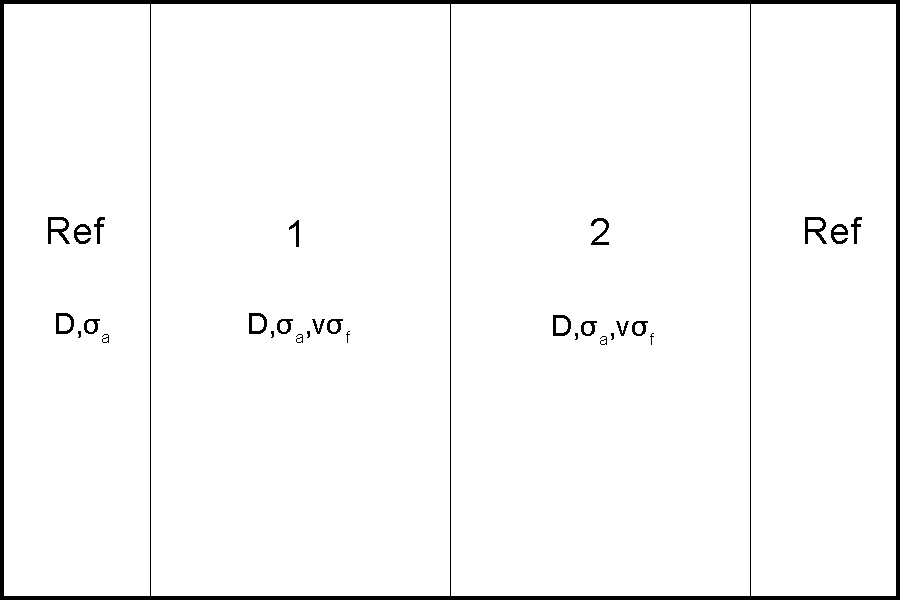
\includegraphics[width=0.7\linewidth]{c5g7/geom}
  \caption{C5G7 Geometry}
  \label{fig:c5g7 geom}
\end{figure}
\begin{figure}[htb]
  \centering
  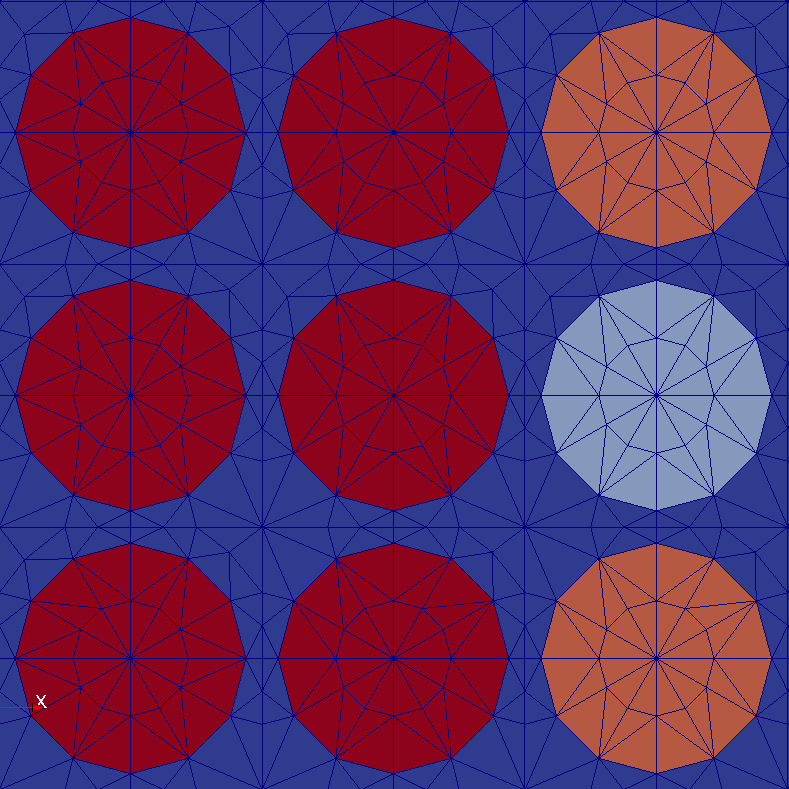
\includegraphics[width=0.7\linewidth]{c5g7/mesh}
  \caption{C5G7 Mesh}
  \label{fig:c5g7 mesh}
\end{figure}
\begin{figure}[htb]
  \centering
  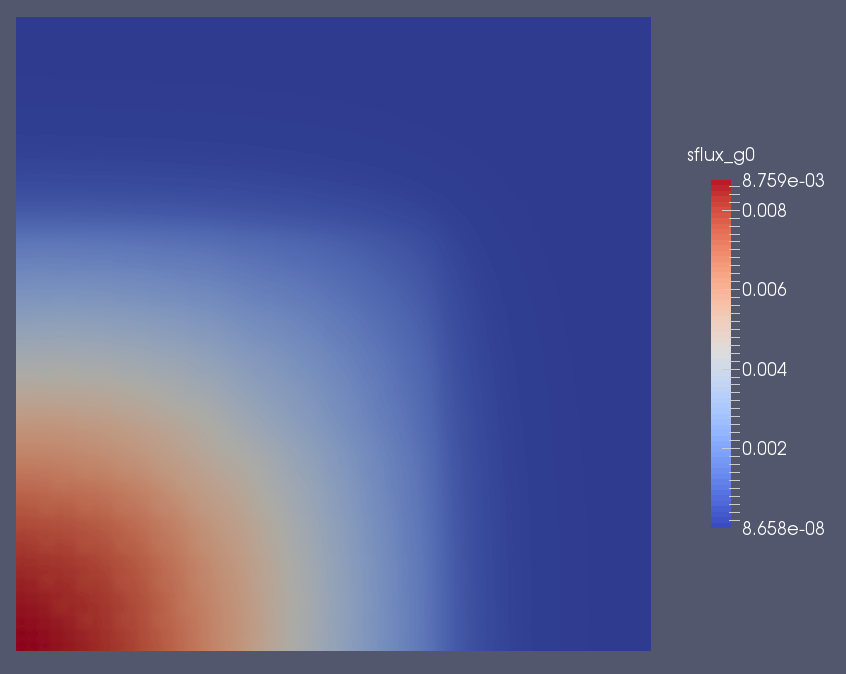
\includegraphics[width=0.7\linewidth]{c5g7/flux0}
  \caption{C5G7 Group 1 (Fast) Flux}
  \label{fig:c5g7 flux0}
\end{figure}
\begin{figure}[htb]
  \centering
  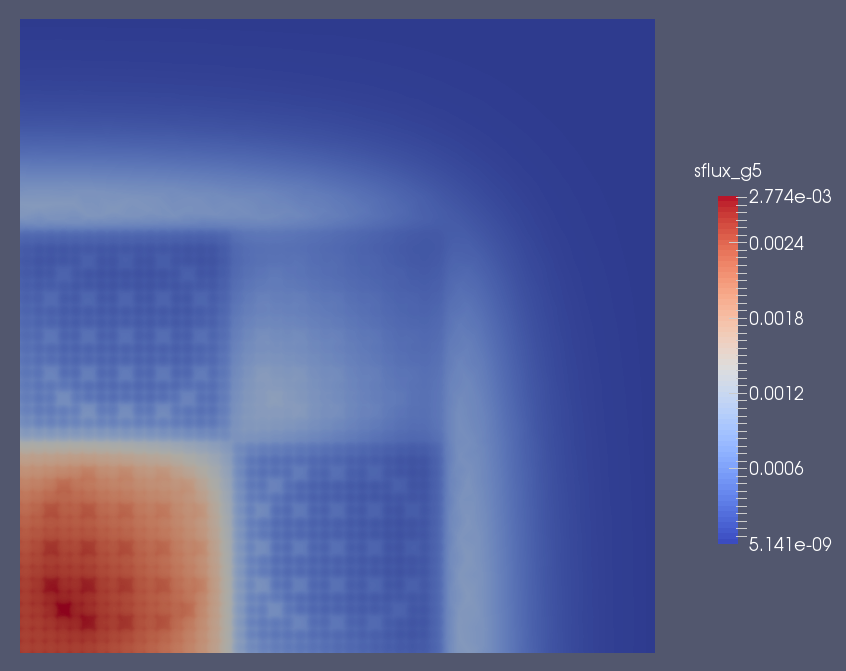
\includegraphics[width=0.7\linewidth]{c5g7/flux5}
  \caption{C5G7 Group 5 (Thermal) Flux}
  \label{fig:c5g7 flux1}
\end{figure}

\begin{table}
  \centering{}
  \begin{tabular}{c c}
    Group & Upper Energy Bound \\ \hline
    7 & 0.02 eV\\
    6 & 0.1 eV\\
    5 & 0.625 eV\\
    4 & 3 eV\\
    3 & 500 keV \\
    2 & 1 MeV \\
    1 & 20 MeV
  \end{tabular}
  \caption{C5G7 Energy Groups}
  \label{tab:c5g7 energy}
\end{table}
This problem is solved using \moose{}-based application \rattlesnake{} \cite{rattlesnake} using the diffusion
equation as the driving physics.  The flux field parameter is set to use first-order Lagrange polynomials to
interpret the finite element space.  For this problem \rattlesnake{} parallelizes quite effectively up to 6
MPI processes, at which point on the Idaho National Laboratory supercomputing framework \texttt{FALCON} each
run takes approximately one minute to converge using \moose{}'s preconditioned Jacobian-free Newton Krylov
solver.

\subsection{Uncertainty}
There are a total of 168 correlated macroscopic cross sections as uncertain inputs to this problem.  To
introduce uncertainty in these cross sections, we use the nominal reference case cross sections as the mean
values of the distributions, and assign a standard deviation of five percent to all inputs.  We also assign
correlations between cross sections of the same type and material but different energy groups, as well as
correlations between cross sections of the same energy group and material but different types.  The
correlation we assign is ten percent.  This approximation could be improved by using uncertainty propagation
on a cross section generation tool to calculate actual covariances; however, for demonstration purposes, using
these assignments is sufficient.

We consider three responses: the $k$-eigenvalue, and the thermal and fast ($g=1,5$) scalar flux measured in the
bottom-left element in the mesh, which corresponds to the center of the reactor.  In order to provide an
orthogonal and reasonably-sized uncertainty space, we first perform a Karhunen-Loevre (KL) \cite{karhunen}
expansion.  This results in a surrogate input space made up of orthogonal, standard normally-distributed
variables.  We refer to the collection of surrogate input variables as \emph{latent} variables, which are
labeled only by their ranking in the KL expansion.  For example, \texttt{latent\_6} is the sixth dimension in
the KL expansion.  The original input space we designate the \emph{manifest} input space, as these are the
inputs manifested to the simulation model.  This follows the naming convention in \raven{}.

We then perform a sensitivity analysis of the responses to the latent inputs using ten thousand Monte Carlo samples.  
The sensitivity values and KL
eigenvalues are used together to construct an importance index, ranking the impact of each latent variable on
both the input and response spaces.  The KL expansion and sensitivity ranking, along with importance
determination, are utilities we use in \raven{}'s toolkit.  The first several importance-ranked eigenvalues
for each response are shown in Table \ref{tab:c5g7 importance}.  There are many latent input dimensions common
in the first several importance rankings for each variable; in particular, latent dimensions 24, 9, 0, and 17
are common to all three, while additionally 10 is common to both the flux terms.  We elect to truncate the
latent input space to include these common terms plus dimension 116 (important to the group 1 flux) and
dimensions 100 and 13 (important to the group 5 flux).  In total this gives our reduced input space a
dimensionality of eight.

\begin{table}
  \centering
  \begin{tabular}{|c|c c|c c|c c|} \hline
    & \multicolumn{2}{|c|}{$k$-eigenvalue} & \multicolumn{2}{|c|}{Center Flux, $g=1$} &
             \multicolumn{2}{|c|}{Center Flux, $g=5$} \\ \hline
    Rank & Dimension & Importance & Dimension & Importance & Dimension & Importance \\ \hline 
    1 &  24 & 0.09606 &  24 & 0.07231 &  24 &  0.07032  \\
    2 &   9 & 0.08555 &   9 & 0.06472 &   9 &  0.06648  \\
    3 &   0 & 0.06861 &   0 & 0.04856 & 100 &  0.06474  \\
    4 &  17 & 0.04737 & 116 & 0.03472 &  13 &  0.03396  \\
    5 &  23 & 0.03415 &  17 & 0.06470 &   0 &  0.03092  \\
    5 & 158 & 0.03047 &  10 & 0.02726 &  17 &  0.02716  \\
    6 & 164 & 0.02852 &   8 & 0.02468 &  10 &  0.02651  \\
    7 &  50 & 0.02695 & 164 & 0.02174 & 118 &  0.02600  \\
    7 &   6 & 0.02315 &  20 & 0.02157 & 117 &  0.02420  \\
  \hline \end{tabular}
  \caption{C5G7 Importance Ranking}
  \label{tab:c5g7 importance}
\end{table}

The agreement for the mean and standard deviation of the original full input space and the truncated latent
space are given in Figure TODO. Both the mean and standard deviation for each the original and reduced space
are calculated using ten thousand Monte Carlo samples, and the error bars given encompass the 95\% confidence
interval for the metric.  TODO discuss agreement.

Since the efforts in this demonstration are to establish the effectiveness of collocation-based methods for
this model, we consider agreement between collocation models and the reduced-space Monte Carlo statistics only.
It is beyond the scope of this work to consider the efficiency of the importance ranking algorithms in
\raven{}.


\section{Results}
Todo, intro to results

\subsection{$k$-Eigenvalue}
As can be seen in Figures TODO, even linear polynomials are sufficient to quite accurately capture the first
two statistical moments of the $k$-eigenvalue for this model.  This suggests a strongly linear dependence of
$k$ on cross sections, which can be justified through analyzing the first derivatives Eq. \ref{eq:diffusion}
with respect to each cross section independently.  This means that any of the collocation methods are very
well-suited to represent the original model, and a cost of far less computational solves than traditional
Monte Carlo.

\subsection{Center Flux, $g=1$}
Todo.

\subsection{Center Flux, $g=5$}
Todo.

\section{Conclusion}
